\begin{abwframe}
\node[anchor=north west,inner sep=0pt,outer sep=0pt] at (40.625,-55.791) {\begin{minipage}[t][69.584bp][c]{878.75bp}\setlength{\parindent}{0pt}\setlength{\parskip}{0pt}{\TimesNR\fontsize{44}{49.28}\selectfont\color{cBC0031}\bfseries\raggedright Example: The NOT Perceptron\par}\end{minipage}};
\node[anchor=north west,inner sep=0pt,outer sep=0pt] at (40.625,-158.857) {\begin{minipage}[t][294.114bp][c]{348.035bp}\setlength{\parindent}{0pt}\setlength{\parskip}{0pt}{\TimesNR\fontsize{24}{26.88}\selectfont\color{c000000}\raggedright Suppose we use the step function for activation.\par}{\TimesNR\fontsize{24}{26.88}\selectfont\color{c000000}\vphantom{Ag}\par}{\TimesNR\fontsize{24}{26.88}\selectfont\color{c000000}\raggedright Suppose Boolean value false is represented as number 0.\par}{\TimesNR\fontsize{24}{26.88}\selectfont\color{c000000}\vphantom{Ag}\par}{\TimesNR\fontsize{24}{26.88}\selectfont\color{c000000}\raggedright Suppose Boolean value true is represented as number 1.\par}{\TimesNR\fontsize{24}{26.88}\selectfont\color{c000000}\vphantom{Ag}\par}{\TimesNR\fontsize{24}{26.88}\selectfont\color{c000000}\raggedright Then, the perceptron on the right computes the Boolean NOT function!\par}\end{minipage}};
\node[anchor=north west,inner sep=0pt,outer sep=0pt] at (56.693,-499.702) {\begin{minipage}[t][11.952bp][c]{324bp}\setlength{\parindent}{0pt}\setlength{\parskip}{0pt}{\TimesNR\fontsize{10}{11.2}\selectfont\color{c7F7F7F}\raggedright Analytics for a Better World Lecture 2\par}\end{minipage}};
\node[anchor=north west,inner sep=0pt,outer sep=0pt] at (880.898,-499.702) {\begin{minipage}[t][11.952bp][c]{22.409bp}\setlength{\parindent}{0pt}\setlength{\parskip}{0pt}{\TimesNR\fontsize{10}{11.2}\selectfont\color{c7F7F7F}\bfseries\raggedleft 24\par}\end{minipage}};
\node[anchor=north west,minimum width=191.123bp,minimum height=65.433bp,inner sep=0pt,fill=none,draw=c000000,line width=0.75bp] at (669.612,-64.446) {};
\node[anchor=north west,inner sep=0pt,outer sep=0pt] at (676.812,-68.046) {\begin{minipage}[t][58.233bp][t]{176.723bp}\setlength{\parindent}{0pt}\setlength{\parskip}{0pt}{\TimesNR\fontsize{24}{26.88}\selectfont\color{c000000}\bfseries\raggedright NOT false = true\par}{\TimesNR\fontsize{24}{26.88}\selectfont\color{c000000}\bfseries\raggedright NOT true = false\par}\end{minipage}};
\draw[fill=cD2CFD5,fill opacity=1,draw=c141215,line width=1bp,rotate around={0:(715.027,-263.628)}] (715.027,-263.628) ellipse [x radius=112.79bp,y radius=61.5bp];
\node[anchor=north west,inner sep=0pt,outer sep=0pt] at (609.437,-205.728) {\begin{minipage}[t][115.8bp][c]{211.18bp}\setlength{\parindent}{0pt}\setlength{\parskip}{0pt}{\TimesNR\fontsize{28}{31.36}\selectfont\color{c000000}\itshape\centering \ensuremath{z}=\ensuremath{h}  \ensuremath{\mathbf{w}} \ensuremath{T} \ensuremath{\mathbf{x}} \par}\end{minipage}};
\draw[fill=none,draw=cFF0000,line width=3bp,-{Stealth}] (435.291,-138.361) -- (635.273,-220.141);
\draw[fill=none,draw=c1F1D21,line width=3bp,-{Stealth}] (432.585,-262.563) -- (602.237,-263.628);
\node[anchor=north west,inner sep=0pt,outer sep=0pt] at (390.922,-245.564) {\begin{minipage}[t][33.998bp][t]{34.463bp}\setlength{\parindent}{0pt}\setlength{\parskip}{0pt}{\TimesNR\fontsize{28}{31.36}\selectfont\color{c000000}\itshape\raggedright  \ensuremath{x} 1 \par}\end{minipage}};
\node[anchor=north west,inner sep=0pt,outer sep=0pt] at (391.829,-100.762) {\begin{minipage}[t][33.998bp][t]{86.925bp}\setlength{\parindent}{0pt}\setlength{\parskip}{0pt}{\TimesNR\fontsize{28}{31.36}\selectfont\color{c000000}\itshape\raggedright  \ensuremath{x} 0 =1\par}\end{minipage}};
\node[anchor=north west,inner sep=0pt,outer sep=0pt,rotate=-21.765] at (503.796,-145.314) {\begin{minipage}[t][33.998bp][t]{92.701bp}\setlength{\parindent}{0pt}\setlength{\parskip}{0pt}{\TimesNR\fontsize{28}{31.36}\selectfont\color{c000000}\itshape\raggedright  \ensuremath{w} 0 =1\par}\end{minipage}};
\node[anchor=north west,inner sep=0pt,outer sep=0pt] at (453.415,-225.447) {\begin{minipage}[t][33.998bp][t]{113.128bp}\setlength{\parindent}{0pt}\setlength{\parskip}{0pt}{\TimesNR\fontsize{28}{31.36}\selectfont\color{c000000}\itshape\raggedright  \ensuremath{w} 1 =\ensuremath{-}2\par}\end{minipage}};
\draw[fill=none,draw=c1F1D21,line width=3bp,-{Stealth}] (827.817,-263.628) -- (936.492,-263.628);
\node[anchor=north west,inner sep=0pt,outer sep=0pt] at (829.425,-224.53) {\begin{minipage}[t][33.998bp][t]{110.564bp}\setlength{\parindent}{0pt}\setlength{\parskip}{0pt}{\TimesNR\fontsize{28}{31.36}\selectfont\color{c000000}\raggedright Output: \ensuremath{z}\par}\end{minipage}};
\node[anchor=north west,inner sep=0pt,outer sep=0pt] at (446.215,-359.39) {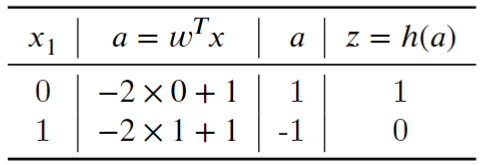
\includegraphics[width=361.55bp,height=123.767bp]{assets/source/slide-24-object-007.png}};
\end{abwframe}
